\section{Baking in the tropics}

Depending on the temperature your fermentation speed adapts.
In a warmer environment everything is faster. In a colder
environment everything is slower.

This includes the speed at which your sourdough ferments
the dough but also the speed of enzymatic reactions. The
amylase and protease enzymes work faster, making more
sugars available and degrading the gluten proteins.

At around 22°C in my kitchen my bulk fermentation is ready
after around 10 hours. I am using around 20 percent of sourdough
starter based on the flour. In summer times the temperatures
in my kitchen sometimes increase to 25°C. In that case
I am reducing the sourdough starter to around 10 percent.
If I wouldn't do that my fermentation would be done after
around 4-7 hours. The problem is that the dough is quite
unstable when fermenting at this high speed. This means
that you are easily running into issues of overfermentation.
Finding the perfect sweet spot between fermenting enough
and not too much is becoming much harder. Normally you might
have a time window of 1 hour. But at the rapid speed it
might be reduced to a time window of 20 minutes. Now at
30°C ambient temperature things are way faster. Your bulk
fermentation might be complete in 2-4 hours when using
10-20 percent starter. Proofing your dough in the fridge
becomes almost impossible. As your dough cools down in the
fridge the fermentation also slows down. However cooling the
dough down from 30°C to 4-6°C in your fridge takes much
longer. Your dough is much more active compared to a dough
that starts at a temperature of 20-25°C. You might
end up overproofing your dough if you leave it overnight
in the fridge.

That's why I recommend that you reduce the amount of starter
that you use in the tropics to something at around 1-5 percent
based on the flour. This will slow down the fermentation
process significantly and provides you a bigger window
of time. Try to aim for an overall bulk fermentation of at
least 8-10 hours. Reduce the amount of starter to get there.

When making a dough try to use the same water temperature
as your ambient temperature. Assuming that the temperature
will climb to 30°C, try to start your dough directly
with 30°C water. This means that you can carefully rely on
a small fermentation probe that visualizes your fermentation
progress. The probe only works reliably if your dough temperature
is equal to your ambient temperature. Else the sample heats
up or cools down faster. So tread carefully when using
the sample in this case. It's always better to stop
the fermentation a little too early rather than too late.
Stretch and folds during the bulk fermentation
will help you to develop a better look and feel for
the dough. An expensive but possibly useful tool
could be a pH meter that allows you to perfectly
measure how much acidity has been created by the
lactic and acetic acid bacteria. In this case measure
the pH repeatedly and figure out a value that works
for your sourdough. In my case I tend to end bulk
fermentation at a pH of around 4.1. Please don't just
follow my pH value, it's very individual. Keep measuring
with different doughs to find out a value that works for you.

\section{My bread stays flat}

A flat bread is in most cases related to your gluten
network breaking down fully. This is not bad, this
means you are eating a fully fermented food. However
from a taste and consistency perspective it might be
that your bread tastes too sour, or is not fluffy anymore.
Please also note that you can only make bread with
great oven spring when making wheat based doughs. When
starting with this hobby I always wondered why my rye
breads would turn out so flat. Rye has gluten yes, but
small particles called {\it hemicelluloses} (arabinoxylan and beta-glucan) \cite{rye-defects}.
prevent the dough from developing a gluten network like you can
do with wheat. Your efforts are in vain, your dough will
stay flat. Only spelt and wheat based doughs have the capability
to retain the \ch{CO2} created by the fermentation.

In most cases something is probably off with your
sourdough starter. This very often happens when the starter
is still relatively young and hasn't yet matured
at fermenting flour. Over time your sourdough
starter is going to become better and better at fermenting
flour. Keep your sourdough starter at room temperature
and then apply daily feedings with a 1:5:5 ratio.
This would be 1 part old starter, 5 parts flour,
5 parts water. This allows you to achieve a better
balance of yeast and bacteria in your sourdough.
Even better could be the use of a stiff sourdough
starter. The stiff sourdough starter boosts
the yeast part of your starter. This allows you
to have less bacterial fermentation, resulting
in a stronger gluten network towards the end
of the fermentation \cite{stiff+starter}. Please
also refer to the section ~\ref{sec:overfermented-dough} where
I explained more about overfermented doughs. You can also
refer to section ~\ref{section:stiff-starter} with more details on
making a stiff sourdough starter.

Furthermore a stronger flour containing more gluten
will help you to push the fermentation further. This
is because your flour contains more gluten and will
take longer to be broken down by your bacteria. Ultimately
if fermented for too long your dough is also going
to be broken down and will become sticky and flat.

To debug whether the excess bacterial fermentation is the issue,
simply taste your dough. Does it taste very sour? If yes,
that's a good indicator. When working the dough, does it
suddenly become very sticky after a few hours? That's a
another good indicator. Please also use your nose to note
the smell of the dough. It shouldn't be too pungent.

\section{I want more tang in my bread}

To achieve more tang in your sourdough bread you have
to ferment your dough for a longer period of time.
Over time the bacteria will metabolize most of the
ethanol created by the yeast in your dough. The bacteria
mostly produces lactic and acetic acid. Lactic acid
is chemically more sour than acetic acid but sometimes
not achieved as sour. In most cases a longer fermentation
is what you want. You will either need to utilize a loaf
pan to make your dough or use a flour that can withstand
a long fermentation period. A flour like this is typically
called a {\it strong flour}. Stronger flours tend
to be from wheat varieties that have be grown in more
sunny conditions. Because of that stronger flours tend
to be more expensive. For freestanding loaves I recommend
to use a flour that contains at least 12 percent protein.
Generally the more protein the longer you can ferment your dough.

Another option to achieve a more sour flavor could be to
use a starter that produces more acetic acid. Acetic acid
bacteria tend to be more common in rye starters (source needed).
Chemically the acetic acid isn't as sour, but when tasting
it will seem more sour. Make sure to use a starter that is at
a hydration of around 100 percent. Acetic acid production
requires oxygen. A too liquid starter tends to favor lactic
acid production because the flour is submerged in water, no
oxygen can reach the fermentation after a while.

\begin{figure}[!htb]
  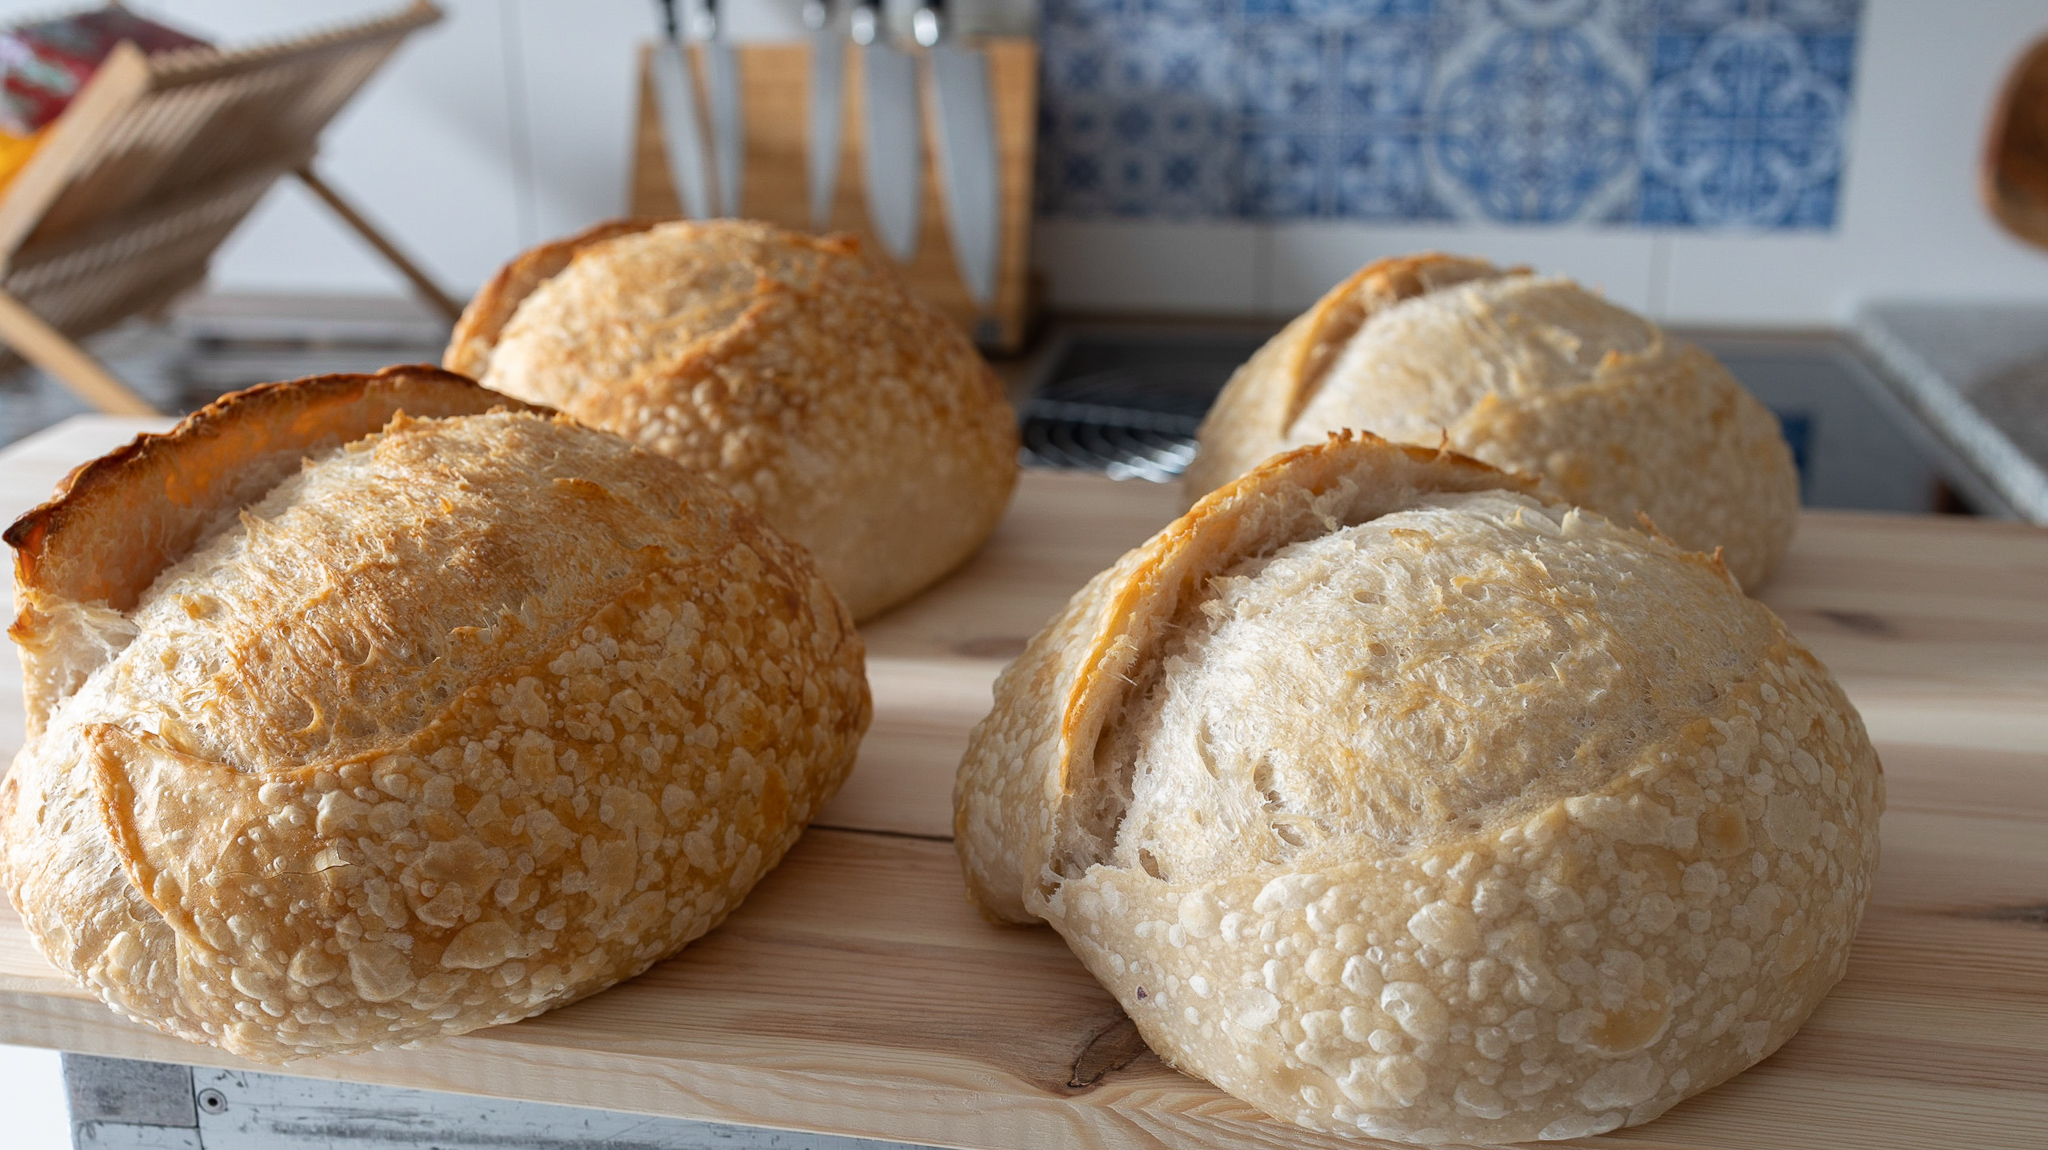
\includegraphics[width=\textwidth]{parbaked-bread.jpg}
  \caption{A half-baked bread, known as "parbaked".}
  \label{fig:parbaked-bread}
\end{figure}

Another more easier option could be to bake your sourdough
twice. I have observed this when shipping bread for my micro
bakery. The idea was to bake my bread for around 30 minutes
until it's sterilized, let it cool down and then ship it
to customers. Once you receive it you just bake it again
for another 20-30 minutes to achieve the desired crust and
then you can eat it. Some of the customers reported a very sour
tasting bread. After investigating a bit more it became
crystal clear. By baking the bread twice you don't boil
as much of the acid during the baking process. Water
evaporates at around 100°C while acetic acid boils at
118°C and lactic acid at 122°c. After baking for 30 minutes
at around 230°C some of the water has started to evaporate,
but not all the acid yet. If you were to continue to bake more
and more of the acid would start to evaporate. Now if you were
to stop baking after 30 minutes, you would typically have reached
a core temperature of around 95°C. Your dough would need
to be cooled down again to room temperature. The crust would
still be quite pale. Then A couple of hours later you start
to bake your dough again. Your crust would become nice and
dark featuring delicious aroma. The aroma is coming from the
maillard reaction. However the core of your dough still won't
exceed the 118°C required to boil the acid. Overall your
bread will be more sour. The enhanced acidity also helps
to prevent pathogens from entering your bread. The bread
will be good for a longer period of time. That's why
the concept of a delivery works well with sour sourdough bread.
In my experiments the bread stayed good for up to a week
in a plastic bag.

\section{My bread is too sour}

Some people like the bread less sour as well. This
is personal preference. To achieve a less sour bread
you need to ferment for a shorter period of time.
The yeast produces \ch{CO2} and ethanol. Both yeast and
bacteria consume the sugars released by the amylase enzyme
in your dough. When the sugar is rare bacteria starts to
consume the leftover ethanol by the yeast. Over time more
and more acidity is created making a more sour dough.

Another angle at this would be to change the yeast/bacteria
ratio of your sourdough. You can start the fermentation with
more yeast and less bacteria. This way for the same given
volume increase of your dough you will have less acidity.
A really good trick is to make sure that you feed your starter
once per day at room temperature. This way you shift
the tides of your starter towards a better yeast fermentation \cite*{more+active+starter}.

To shift the tides even further a real game changer
to me has been to create a stiff sourdough starter. The
stiff sourdough starter is at a hydration of around 50 percent.
By doing so your sourdough starter will favor yeast
activity a lot more. Your doughs will be more fluffy and will
not as sour for a given volume increase. I tested this
by putting condoms over different glas jars. I used
the same amount of flour for each of the samples.
I tested a regular starter, a liquid starter and a stiff
starter. The stiff starter by far created the most \ch{CO2}
compared to the other starters. The balloons were inflated
the most. \cite{stiff+starter}

Another non conventional approach could be to add baking
powder to your dough. The baking powder neutralizes the
lactic acid and will make a much milder dough.\cite{baking+powder+reduce-acidity}

\section{Fixing a moldy sourdough starter}

First of all - making a moldy sourdough starter is very difficult.
It's an indicator that something might be completely off in your starter.
Normally the symbiosis of yeast and bacteria does not allow external
pathogens such as mold to enter your sourdough starter.
The low pH created by the bacteria is a very hostile environment
that no other pathogens like. Generally everything below a pH
of 4.2 can be considered food safe\cite{food+safe+ph}. This
is the concept of pickled foods. And your sourdough bread
is essentially pickled bread.

I have seen this happening especially when the sourdough
starter is relatively young. Each flour naturally contains
mold spores. When beginning a sourdough starter all
the microorganisms start to compete by metabolizing the
flour. Mold can sometimes win the race and out compete
the natural wild yeast and bacteria. In that case simply
try cultivating your sourdough starter again. If it molds
again it might be a very moldy batch of flour. Try a different
flour to begin your sourdough starter with.

Mature sourdough starters should not mold unless the conditions
of the starter change. I have seen mold appearing when the starter is stored
in the fridge and the surface dried out. Also sometimes on the
edges of your starter's container. Typically in areas where no active
starter microorganisms can reach. Simply try to extract an
area of your starter that has no mold. Feed it again with flour and
water. After a few feedings your starter should be back to normal.
Take only a tiny bit of starter. 1-2 grams are enough. They already
contain millions of microorganisms.

Mold favors aerobic conditions. This means that air is required in order
for the mold fungus to grow. Another technique that has worked for me
was to convert my sourdough starter into a liquid starter. This successfully
shifted my starter from acetic acid production to lactic acid production.
Acetic acid similarly to mold requires oxygen to be produced. After
submerging the flour with water over the time the lactic acid bacteria
out competed the acetic acid bacteria. This is a similar concept to pickled
foods. By doing this you are essentially killing all alive mold fungi. You
might only have some spores left. With each feeding the spores will become
less and less. Furthermore it seems that lactic acid bacteria produce
metabolites that inhibit mold growth. \cite{mold+lactic+acid+bacteria}

\begin{figure}[!htb]
  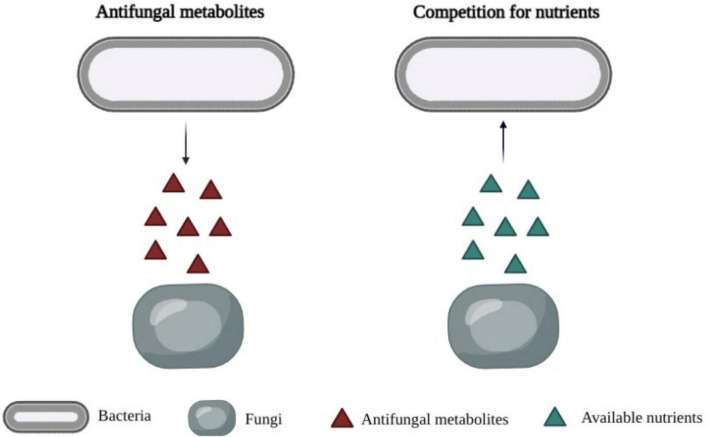
\includegraphics[width=\textwidth]{fungi-lactic-acid-interactions}
  \caption{The interaction of lactic acid bacteria and mold fungi.
           The authors Ce Shi et al. show how bacteria are producing
           metabolites that inhibit fungus growth. \cite{mold+lactic+acid+bacteria}}
  \label{fig:fungi-lactic-acid-interactions}
\end{figure}

To pickle your starter simply take a bit of your existing starter (5 grams for
instance). Then feed the mixture with 20g of flour and 100g of water. You have
created a starter a hydration of around 500 percent. Shake the mixture vigorously.
After a few hours you should start seeing most of the flower near the bottom
of your container. After a while most of the oxygen from the bottom mixture
is depleted and anaerobic lactic acid bacteria will start to thrive. Take a
note of the smell your sourdough starter. If it was previously acetic
it will now change to be a lot more dairy. Extract a bit of your mixture the
next day by shaking everything first. Take 5g of the previous mixture, feed
again with another 20g of flour and another 100g of water. After 2-3
additional feedings your starter should have adapted. When switching back
to a hydration of 100 percent the mold should have been eliminated. Please note that
more tests should be conducted on this topic. It would be nice to really
carefully analyze the microorganisms before the pickling and after.

\section{My bread flattens out removing it from the banneton}

After removing your dough from the banneton your dough will always
flatten out a bit. That's because over time your gluten network
relaxes and can no longer hold the shape. However, during the course
of baking your dough is going to increase in size and inflate again.

If your dough however flattens out completely it's a sign that
you have fermented your dough for too long. Please refer to ~\ref{sec:overfermented-dough}
where I explain about overfermented doughs. Your bacteria
has consumed most of your gluten network. That's why your
dough fully collapses and stays flat during the bake. The
\ch{CO2} and evaporating water will diffuse out of the dough.
A related symptom is that your dough sticks to the banneton.
When starting baking I combatted this with rice flour.
It works but might be a false friend. I gently rub my
dough with a bit of non-rice flour before placing it in
the banneton. Now then the dough starts to stick to the banneton
while I remove it I resort to a drastic measure. I immediately
grease a loaf pan and directly place the dough inside. The loaf
pan provides a barrier and the dough can't flatten out as much.
The dough won't be as fluffy but super delicious if you love tangy bread.

If you own a pH meter take a note of your dough's pH before baking.
This will allow you to better judge your dough throughout
the fermentation process.

\section{My bread flattens out during shaping}

Similarly to a dough flattening out after removing it from the banneton,
a flattened dough after shaping is also a possible sign of overfermentation.

When you try to shape the dough, can you easily tear pieces from the dough?
If yes, you have definitely overfermented your dough. If not it might just
be a sign that you have not created enough dough strength for your dough.
A ciabatta for instance is a dough that tends to flatten out a bit after shaping.

If your dough is not possible to be shaped at all use a greased loaf pan
to rescue your dough. You can also cut a piece of the dough and use it
as the starter for your next dough. Your sourdough dough is essentially
just a gigantic starter.

\section{Liquid on top of my starter}

Sometimes a liquid in many cases black liquid gathers on top
of your sourdough starter. The liquid might have a pungent
smell to it. Many people confuse this with mold. I have seen
bakers recommending to discard the starter because of this liquid.
The liquid is commonly known as {\it hooch}. After a while
of no activity the heavier flour separates from the water. The flour
will sit at the bottom of your jar and the liquid will stay on top.
The liquid turns darker because some particles of the flour weigh
less than the water and float on top. Furthermore dead microorganisms
float in this liquid. This liquid is not a bad thing, it's actively
protecting your sourdough starter from aerobic mold entering through
the top.

\begin{figure}[!htb]
  \centering
  \includegraphics[width=0.5\textwidth]{hooch}
  \caption{Hooch building on top of a sourdough starter. \cite{liquid+on+starter}}
  \label{fig:hooch}
\end{figure}

Simply stir your sourdough starter to homogenize the hooch back
into your starter. The hooch will disappear. Then use a little bit of
your sourdough starter to setup the starter for your next bread.
Once hooch appears your starter has likely fermented for a long
period of time. It might be very sour. This state of starter
is excellent to make discard crackers or a discard bread. Don't throw
anything away. Your hooch is a sign that you have a long fermented
dough in front of you. Compare it to a 2 year ripened Parmigiano cheese.
The dough in front of you is full of delicious flavor.

\section{Why does my starter smell like vinegar or acetone?}

Your sourdough starter has likely produced a lot of acetic acid.
Acetic acid is essential when creating vinegar. Once no additional
food is left some of your starter's bacteria will consume ethanol
and convert it into acetic acid. Acetic acid has a very pungent smell.
When tasting acetic acid the flavor of your bread is often perceived
as quite strong.

\begin{figure}[!htb]
  \centering
  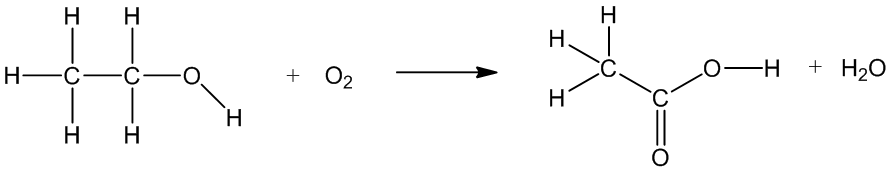
\includegraphics[width=1.0\textwidth]{ethanol-oxidation}
  \caption{Oxygen is required to create acetic acid \cite{acetic+acid+production}.}
  \label{fig:ethanol-oxidation}
\end{figure}

This is nothing bad. But in case you would like to change
the flavor of your final bread consider converting
your sourdough starter into a liquid starter. This will
help to prioritize lactic acid producing bacteria.
Your flavor will change to dairy compared to vinegary.
You can't go back though. After the conversion your starter
will never go back to acetic acid production because you have
changed the tides towards primarily lactic acid fermentation.
I like to have a separate rye starter. In my experiments
rye starters tend to feature many acetic acid bacteria.
This starter is excellent when you want to make a very hearty
strong tasting bread. A pure rye bread tastes excellent when
made with such a starter. The flavor when taking a bite
is incredible. It nicely plays with soups as well. Just take
a bit of this bread and dip it in your soup.

\section{My crust becomes chewy}

Depending on which style of bread you are making a
thick crackly crust is sometimes desired. The crust
of your bread is created during the 2nd stage of the
baking process once the steaming source of your
oven has been removed. The dark colors are created by
the process known as {\it Maillard reaction} and then followed
by another process known as {\it caramelization}. Each
color of crust offers the taster a different aroma.

What happens quite often is that the crust becomes chewy after a day.
Sometimes when baking in the tropics with high humidity the
crust only stays in this stage for a few hours. Afterwards
the crust becomes chewy. It's no longer as crisped compared
to the moment after baking. Your dough still contains moisture.
This moisture will start to homogenize in the final bread and
partially evaporate. The result is that your crust becomes chewy.

Similarly when storing your bread in a container or in a plastic
bag your crust is going to become chewy. I have no fix for this yet.
I typically tend to store my breads in a plastic bag inside of my fridge.
This allows the moisture to stay inside of bread. When taking a slice
I always toast each slice. This way some of the crispness returns.
If you know of a great way please reach out and I will update
this book with your findings.

\section{My dough completely tears after a long fermentation}

Sometimes when touching your dough after a long fermentation
it completely tears apart. This could be for 2 reasons. It might
be that the bacteria completely consumed the gluten of your flour.
On the other hand over time your gluten network automatically
degrades. This is the protease enzyme converting the gluten
network into smaller amino acids the seedling can use as
building blocks for its growth. This process starts to happen
the moment you mix flour and water. The longer your dough sits
the more gluten is broken down. As the gluten holds the
wheat dough together your dough will ultimately tear.

\begin{figure}[!htb]
  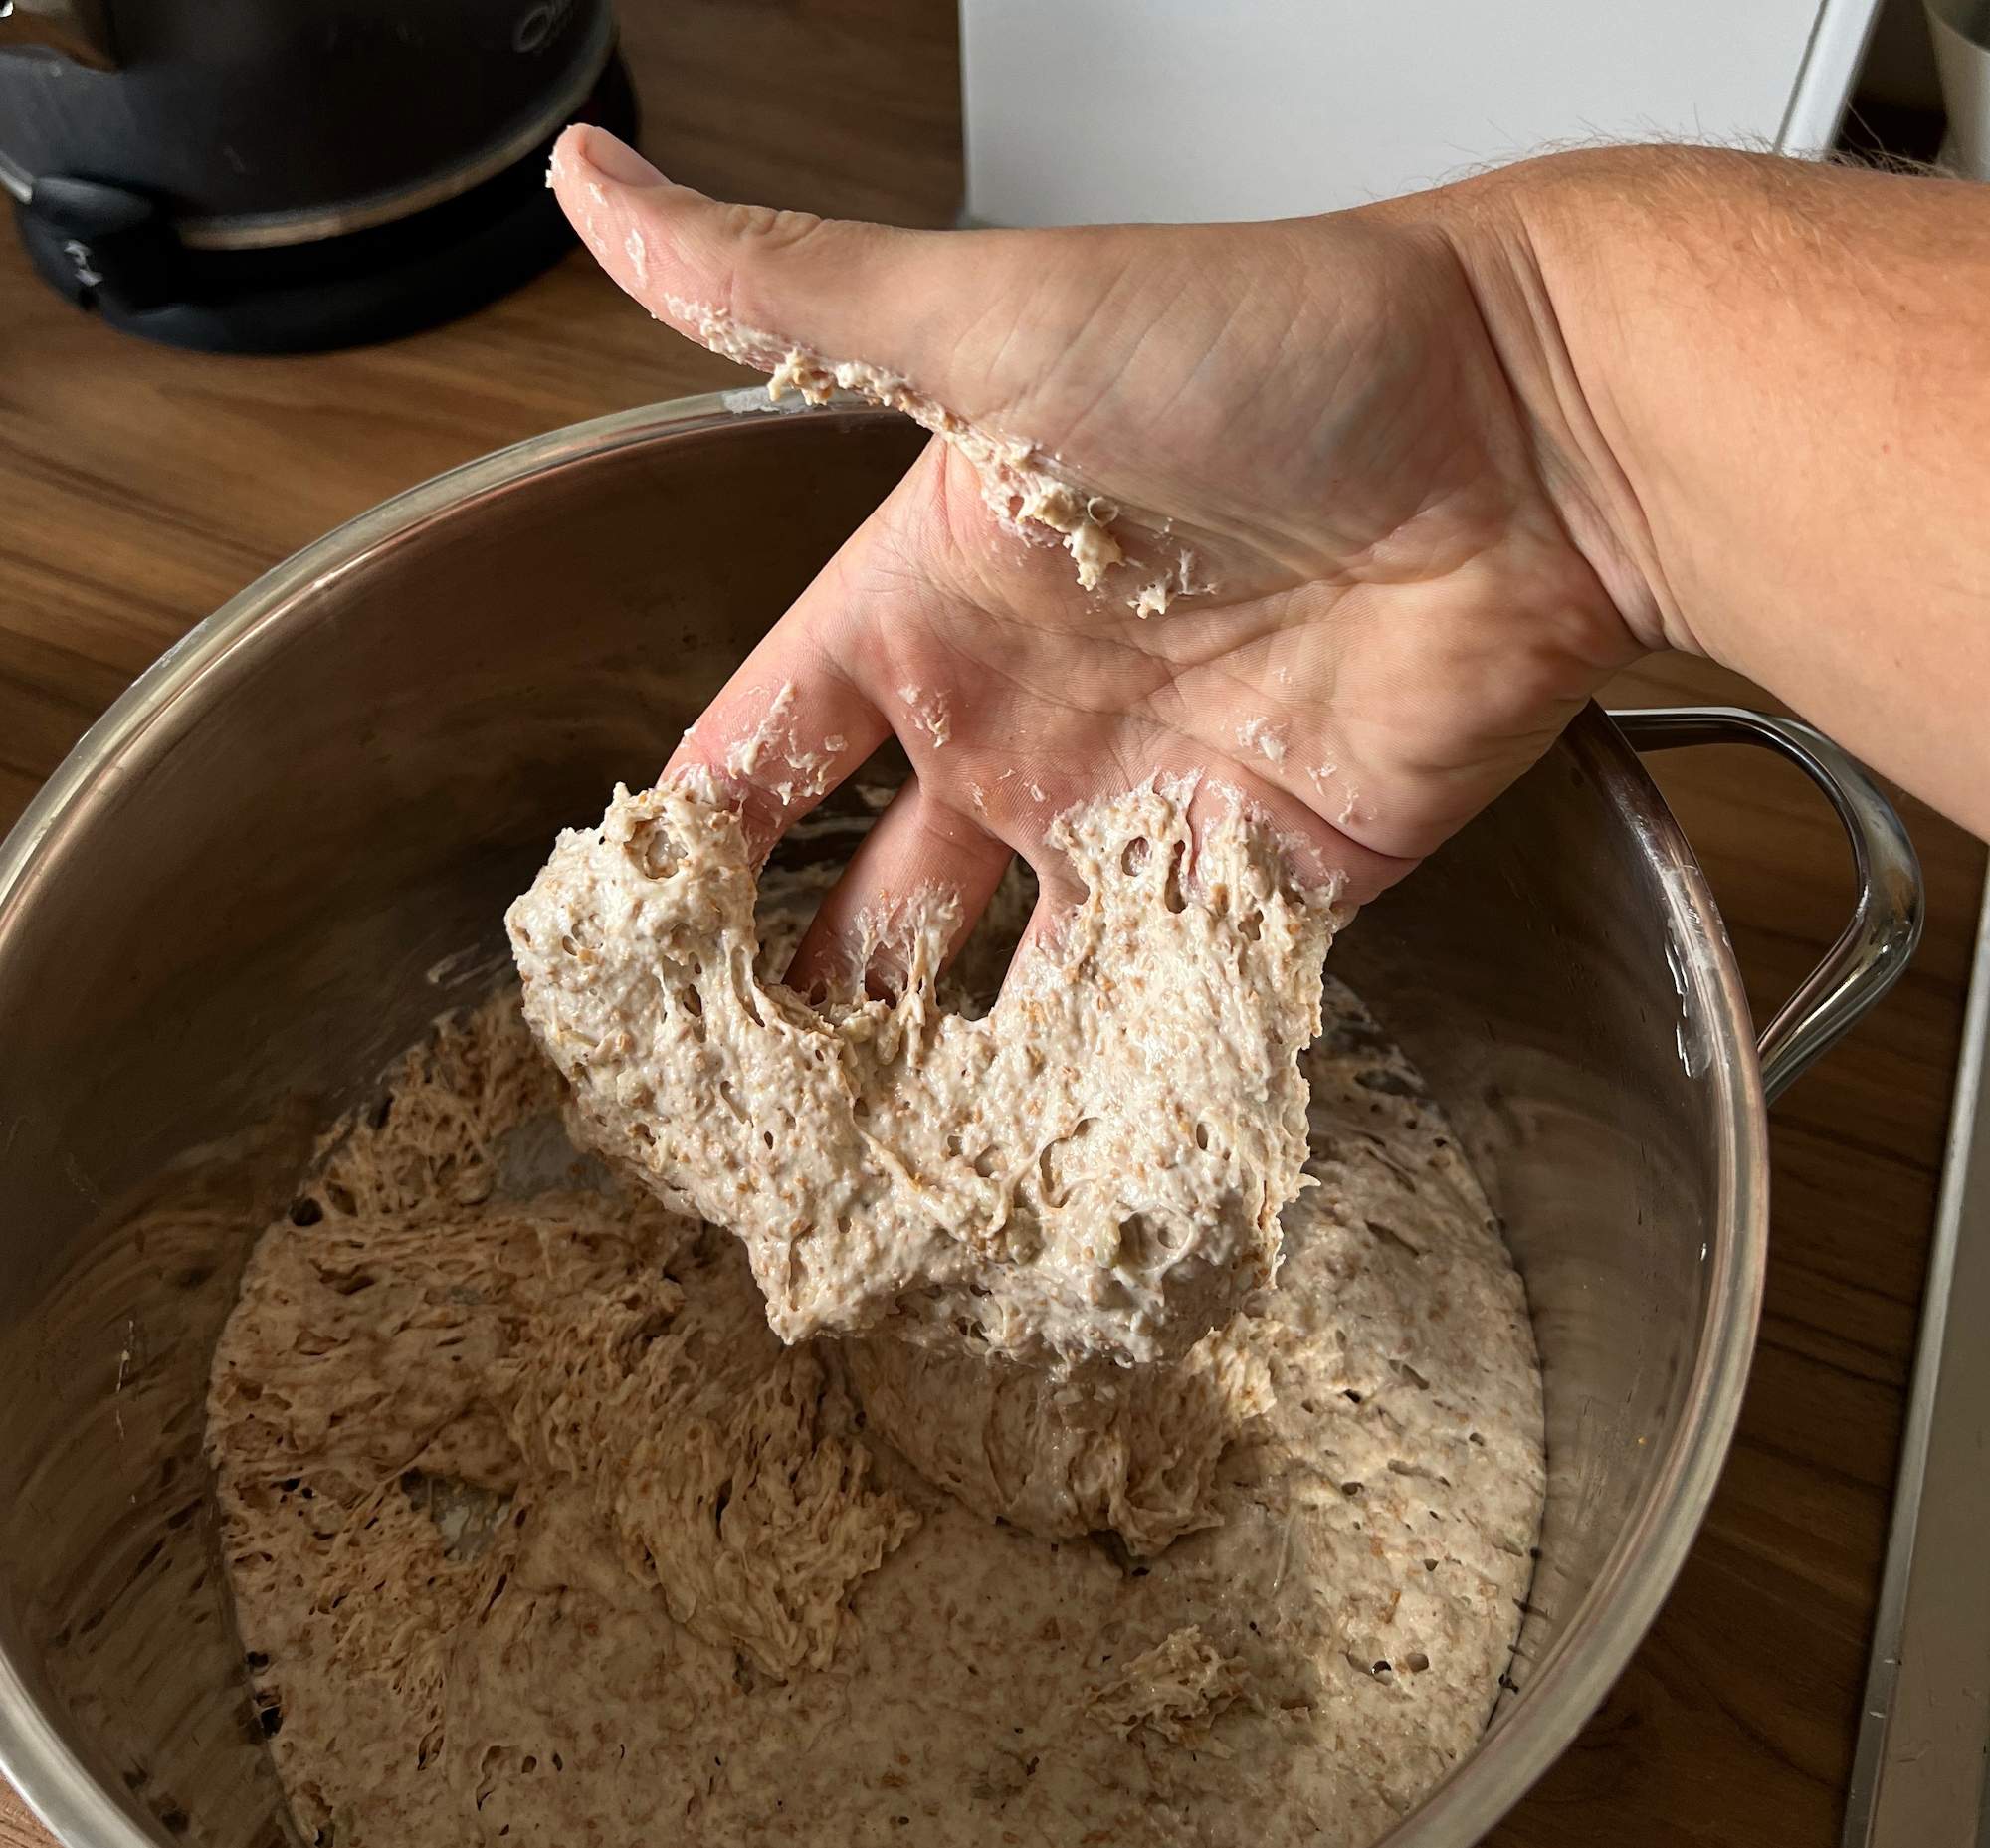
\includegraphics[width=1.0\textwidth]{tearing-dough}
  \caption{My dough tearing after 24 hours of no activity}
  \label{fig:tearing-dough}
\end{figure}

In the picture~\ref{fig:tearing-dough} I experimented with
using a starter that has not been fed for 30 days at room temperature.
I tried to make a dough directly out of the unfed starter.
Typically after a long period
without feedings your microbes start to sporulate and go
into hibernation mode. This way they can survive for a long
period of time without extra feedings. Adding additional food
will activate them again. In this case the dough did not ferment
fast enough before the protease broke down the gluten. By activating
your microbes they will start to reproduce and increase in quantity
for as long as there is food available. But this process
in my case was not fast enough. After around 24 hours the whole
dough just started to completely tear apart. The whole process was further
accelerated by me using whole wheat flour. Whole wheat
contains more enzymes than white flour.

To fix this try to make sure that your sourdough starter is lively
and active. Simply apply a couple of more feedings in advance before
making your dough. This way your dough becomes ready to shape
before it has completely broken down.

\section{My sourdough starter is too sour}

A too sour sourdough starter will cause problems during
the fermentation. Your fermentation will be more on the
bacterial side, rather than the yeast side. This means
you will likely create a more tangy dough which isn't
as fluffy as it could be. The goal is to reach the right
balance: Fluffy consistency from the yeast and a great
not too strong tang from the bacteria. This depends
of course on what you are looking for in terms of taste
in your bread. When making rye bread I prefer to be more
on the tangy side for instance. When the described balance
is off. the first thing to check is your sourdough starter.

Note the smell of your starter. Does it smell very sour?
Taste a bit of your starter too. How sour does it taste?
Over time every starter becomes more and more sour the longer
you wait. But sometimes your starter becomes sour too fast.
In this case apply daily feedings to your starter. Reduce
the amount of old starter that you use to feed. A ratio
of 1:5:5 or 1:10:10 can do wonders. In this case you would
take 1 part of starter (10g) and feed it with 50g of flour
and 50g of water. This way the microorganisms start
the fermentation in a green field environment. This is
similar to the 10 percent starter of 20 percent starter
ratio that you use to make a dough. These days I almost
never use a 1:1:1 ratio. This only makes sense when you
are initially creating your starter. You want a sour
environment so that your microorganisms outcompete
potential pathogens. The acidic environment is toxic
to most pathogens that you do not want in your starter.

Another approach that can help is to convert your
sourdough starter into a stiff starter as
described in section \ref{section:stiff-starter}.

\section{My starter does not double in size}

Some bakers call for the sourdough starter to
double in size before using it.
The idea is to use the sourdough starter at
peak performance to ensure a
balanced fermentation in the main dough.

The doubling in size metric should be
taken with a grain of salt when judging
your starter. Depending on the flour
you use to feed the starter different levels
of its rising can be expected.
For instance, if you use rye flour then only
very little gas from the
fermentation can be retained inside the
starter. In consequence, your
sourdough starter will not rise as much. It
could be in a healthy shape
though. If you use wheat flour with less gluten
the starter will not rise as
much too. The reason is that you have a weaker
gluten network resulting in
more gas dispersing out of your dough.

That being said it is recommended that you develop
your volume increase
metric. Your starter will increase in size and then
ultimately lose structure
and collapse. Observe the point before it collapses.
This is the point when
you should use your starter. This could be a
50 percent volume increase, 100
percent or 200 percent. It is always better to use
the starter a little bit
too early rather than too late. If you use the
starter later reduce the
quantity that you use. If the recipe calls for a 20
percent starter quantity,
use only 10
percent starter in that case. Your starter will
regrow in your main dough.

On top of relying on the size increase start
taking note of your starter's
smell. Over time you will be able to judge its
fermentation state based on the
smell. The stronger the smell becomes the further
your dough has fermented.
This is a sign that you should use fewer starters
when making the actual dough.

Please refer to section \ref{section:readying-starter} "\nameref{section:readying-starter}"
for more information on the topic.

\section{Should I autolyse my dough?}

In 95 percent of all cases, an autolysis
makes no sense. Instead I recommend
that you conduct a fermentolysis. You
can read more about the autolysis process in
section \ref{section:autolysis} and
more about the topic of fermentolysis
in section \ref{section:fermentolysis}.

The fermentolysis combines all the benefits
of the autolysis while eliminating disadvantages
such as having to knead the dough multiple times.

The autolysis only makes sense when you might
bake a fast fermenting yeast-based dough with a
high yeast inoculation rate. But even in that
case you could just lower the amount of yeast
to fermentolyse rather than autolyse.

\section{What's the benefit of using a stiff sourdough starter?}

A regular sourdough starter has equal parts of
flour and water (100 percent hydration). A stiffer
sourdough starter features a hydration level of 50 to 60 percent.

The stiff sourdough starter boosts the yeast part
of your starter more. This way your gluten degrades
slower and you can ferment for a longer period. This
is especially handy when baking with lower gluten flours.

You can read more about the topic of stiff sourdough
starters in section \ref{section:stiff-starter}.

\section{What's the benefit of using a liquid sourdough starter?}

The liquid starter will boost anaerobic bacterial
fermentation in your starter. This way your starter
tends to produce more lactic acid rather than acetic
acid. Lactic acid is perceived as milder and more
yogurty. Acetic acid can sometimes taste quite
pungent.  Acetic acid can be perfect when making 
dark rye bread but not so much when making a fluffy
ciabatta-style loaf.

When converting your starter to a liquid starter you are
permanently altering the microbiome of your starter.
You can not go back once you eliminated acetic
acid-producing bacteria. So it is recommended to keep
a backup of your original starter.

A downside to the liquid starter is the overall
enhanced bacterial activity. This means the baked bread
will have more acidity (but milder). The dough will degrade
faster during fermentation. For this reason, you
will need to use strong high gluten flour when using
this type of starter.

You can read more about the liquid starter
in section \ref{section:liquid-starter}

\section{My new starter doesn't rise at all}

Make sure that you use unchlorinated water.
In many areas of the world tap water has
chlorine added to kill microorganisms. If that's
the case in your region bottled spring water will
help.

Make sure to use whole flour (whole wheat, whole rye, etc.).
These flours have more natural wild yeast and
bacterial contamination. Making a starter
from just white flour sometimes doesn't work.
Try to use organic unbleached flour to make
the starter. Industrial flour can sometimes
be treated too much with fungicides.

\section{I made a starter, it rose on day 3 and now not anymore}

This is normal. As your starter is maturing different
microorganisms are activated. Especially during
the first days of the process bad microbes
like mold can be activated. These cause your
starter to rise a lot. With each subsequent
starter-feeding, you select the microbes that are best
at fermenting flour. For this reason, it is
recommended to discard the leftover unused starter
from the first days of the process. Later on, unneeded
starter amounts should never be thrown away. You can make
great discard bread out of it.

So just keep going and don't give up. The first big
rise is an indicator that you are doing everything
right. Based on my experience it takes around 7
days to grow a starter. As you feed your starter
more and more it will become even better at fermenting
flour. The first bread might not go exactly as you
planned, but you will get there eventually. Each
feeding makes your starter stronger and stronger.

\section{My flour has low gluten content - what should I do?}

You can always mix in a little bit of vital wheat gluten. Vital wheat gluten
is concentrated extracted gluten from wheat flour.

I recommend that you add around 5 grams of wheat gluten for every 100 grams of
flour that you are using.

\section{What's a good level of water (hydration) to make a dough?}

Especially when starting to make bread use lower amounts of water. This will
greatly simplify the whole process. I recommend using a level of around 60
percent hydration. So for every 100 grams of flour use around 60 grams of water.
This ballpark figure will work for most flours. With this hydration, you can
make bread, buns, pizzas, and even baguettes out of the same dough.

With the lower hydration dough handling becomes easier and you have more yeast
fermentation, resulting in lower overfermentation risk.

\section{What's the best stage to incorporate inclusions (seeds) into the dough?}

You can include seeds directly at the start when mixing the dough. If you use
whole seeds such as wheat or rye kernels, soak them in water overnight and
then rinse them before adding them to the dough. This makes sure that they
are not crunchy and soft enough when eating the bread. If you forgot to soak
them you can cook the seeds for 10 minutes in hot water. Rinse them with cold
water before adding them to your dough.

If you want to sweeten the dough your best option is to add sugar during the
shaping stage. Initial sugar is typically fermented and no residual sugar
remains. Adjust your shaping technique a little bit and spread your sugar
mixture over a flattened-out dough. You can then roll the dough together
incorporating layers of sugar.

\section{My dough sample (aliquot) doesn't rise, what's wrong?}

If you see that your dough rises in size but your aliquot doesn't chances
are that both are fermenting at a different speed. This can often
happen when the temperature in your kitchen changes. The aliquot
is more susceptible to temperature changes than the main dough.
Because the sample is smaller in size it will heat up or cool down
faster.

For this reason, you must use room-temperature water when
making your dough. By having the same temperature in both the sample
and your dough you make sure that both ferment at the same rate.

If the temperature in your room changes significantly during the day, your
best option is to use a see-through container. Mark the container to properly
measure your dough's size increase.

Another option could be to use a more expensive pH meter to measure your
dough's acidity buildup. You can read more about different ways of managing
bulk fermentation in section ~\ref{section:bulk-fermentation}.
